%%%%%%%%%%%%%%%%%%%%%%%%%%%%%%%%%%%%%%%%%
% Beamer Presentation
% LaTeX Template
% Version 2.0 (March 8, 2022)
%
% This template originates from:
% https://www.LaTeXTemplates.com
%
% Author:
% Vel (vel@latextemplates.com)
%
% License:
% CC BY-NC-SA 4.0 (https://creativecommons.org/licenses/by-nc-sa/4.0/)
%
%%%%%%%%%%%%%%%%%%%%%%%%%%%%%%%%%%%%%%%%%

%%%%%%%%%%%%%%%%%%%%%%%%%%%%%%%%%%%%%%%%%
% This presentation template is an adaptation of the template mentioned above. It has been created by Giovanni Spadaro and it is available on GitHub (https://github.com/Giovo17/presentation-template-unict-lm-data).
%%%%%%%%%%%%%%%%%%%%%%%%%%%%%%%%%%%%%%%%%

%----------------------------------------------------------------------------------------
%	PACKAGES AND OTHER DOCUMENT CONFIGURATIONS
%----------------------------------------------------------------------------------------

\documentclass[
	11pt, % Set the default font size, options include: 8pt, 9pt, 10pt, 11pt, 12pt, 14pt, 17pt, 20pt
	%t, % Uncomment to vertically align all slide content to the top of the slide, rather than the default centered
	%aspectratio=169, % Uncomment to set the aspect ratio to a 16:9 ratio which matches the aspect ratio of 1080p and 4K screens and projectors
]{beamer}

\graphicspath{{img/}} % Specifies where to look for included images (trailing slash required)

\usepackage{booktabs} % Allows the use of \toprule, \midrule and \bottomrule for better rules in tables

%----------------------------------------------------------------------------------------
%	SELECT LAYOUT THEME
%----------------------------------------------------------------------------------------

% Beamer comes with a number of default layout themes which change the colors and layouts of slides. Below is a list of all themes available, uncomment each in turn to see what they look like.

%\usetheme{default}
%\usetheme{AnnArbor}
%\usetheme{Antibes}
%\usetheme{Bergen}
%\usetheme{Berkeley}
%\usetheme{Berlin}
\usetheme{Boadilla}
%\usetheme{CambridgeUS}
%\usetheme{Copenhagen}
%\usetheme{Darmstadt}
%\usetheme{Dresden}
%\usetheme{Frankfurt}
%\usetheme{Goettingen}
%\usetheme{Hannover}
%\usetheme{Ilmenau}
%\usetheme{JuanLesPins}
%\usetheme{Luebeck}
%\usetheme{Madrid}
%\usetheme{Malmoe}
%\usetheme{Marburg}
%\usetheme{Montpellier}
%\usetheme{PaloAlto}
%\usetheme{Pittsburgh}
%\usetheme{Rochester}
%\usetheme{Singapore}
%\usetheme{Szeged}
%\usetheme{Warsaw}

%----------------------------------------------------------------------------------------
%	SELECT COLOR THEME
%----------------------------------------------------------------------------------------

% Beamer comes with a number of color themes that can be applied to any layout theme to change its colors. Uncomment each of these in turn to see how they change the colors of your selected layout theme.

%\usecolortheme{albatross}
%\usecolortheme{beaver}   % red
%\usecolortheme{beetle}
%\usecolortheme{crane}   % yellow
%\usecolortheme{dolphin}  % purple
%\usecolortheme{dove}   % white
%\usecolortheme{fly}   % grey
%\usecolortheme{lily}   % purple
%\usecolortheme{monarca}   % yellow background and black
%\usecolortheme{seagull}
%\usecolortheme{seahorse}
%\usecolortheme{spruce}   % green
\usecolortheme{whale}
%\usecolortheme{wolverine}

%----------------------------------------------------------------------------------------
%	SELECT FONT THEME & FONTS
%----------------------------------------------------------------------------------------

% Beamer comes with several font themes to easily change the fonts used in various parts of the presentation. Review the comments beside each one to decide if you would like to use it. Note that additional options can be specified for several of these font themes, consult the beamer documentation for more information.

\usefonttheme{default} % Typeset using the default sans serif font
%\usefonttheme{serif} % Typeset using the default serif font (make sure a sans font isn't being set as the default font if you use this option!)
%\usefonttheme{structurebold} % Typeset important structure text (titles, headlines, footlines, sidebar, etc) in bold
%\usefonttheme{structureitalicserif} % Typeset important structure text (titles, headlines, footlines, sidebar, etc) in italic serif
%\usefonttheme{structuresmallcapsserif} % Typeset important structure text (titles, headlines, footlines, sidebar, etc) in small caps serif

%------------------------------------------------

%\usepackage{mathptmx} % Use the Times font for serif text
\usepackage{palatino} % Use the Palatino font for serif text

%\usepackage{helvet} % Use the Helvetica font for sans serif text
\usepackage[default]{opensans} % Use the Open Sans font for sans serif text
%\usepackage[default]{FiraSans} % Use the Fira Sans font for sans serif text
%\usepackage[default]{lato} % Use the Lato font for sans serif text

%----------------------------------------------------------------------------------------
%	SELECT INNER THEME
%----------------------------------------------------------------------------------------

% Inner themes change the styling of internal slide elements, for example: bullet points, blocks, bibliography entries, title pages, theorems, etc. Uncomment each theme in turn to see what changes it makes to your presentation.

%\useinnertheme{default}
\useinnertheme{circles}
%\useinnertheme{rectangles}
%\useinnertheme{rounded}
%\useinnertheme{inmargin}

%----------------------------------------------------------------------------------------
%	SELECT OUTER THEME
%----------------------------------------------------------------------------------------

% Outer themes change the overall layout of slides, such as: header and footer lines, sidebars and slide titles. Uncomment each theme in turn to see what changes it makes to your presentation.

\useoutertheme{default}
%\useoutertheme{infolines}
% \useoutertheme{miniframes}
% \useoutertheme{smoothbars}
%\useoutertheme{sidebar}
%\useoutertheme{split}
%\useoutertheme{shadow}
%\useoutertheme{tree}
%\useoutertheme{smoothtree}

%\setbeamertemplate{footline} % Uncomment this line to remove the footer line in all slides
%\setbeamertemplate{footline}[page number] % Uncomment this line to replace the footer line in all slides with a simple slide count

%\setbeamertemplate{navigation symbols}{} % Uncomment this line to remove the navigation symbols from the bottom of all slides

%----------------------------------------------------------------------------------------
%	PRESENTATION INFORMATION
%----------------------------------------------------------------------------------------

\title[Crittografia]{Presentazione progetto per il corso di Crittografia UNIPR} % The short title in the optional parameter appears at the bottom of every slide, the full title in the main parameter is only on the title page

\author[Ciccarello]{Andrea Ciccarello} % Presenter name(s), the optional parameter can contain a shortened version to appear on the bottom of every slide, while the main parameter will appear on the title slide

\institute[UNIPR]{Università degli studi di Parma} % Your institution, the optional parameter can be used for the institution shorthand and will appear on the bottom of every slide after author names, while the required parameter is used on the title slide and can include your email address or additional information on separate lines

\date[2024]{June 2024} % Presentation date or conference/meeting name, the optional parameter can contain a shortened version to appear on the bottom of every slide, while the required parameter value is output to the title slide

%----------------------------------------------------------------------------------------

\begin{document}

%----------------------------------------------------------------------------------------
%	TITLE SLIDE
%----------------------------------------------------------------------------------------

\begin{frame}

	\begin{figure}
		
\includegraphics[width=0.25\linewidth]{img/logo-unipr/Logo unipr.png}
	\end{figure}

	\titlepage % Output the title slide, automatically created using the text entered in the PRESENTATION INFORMATION block above
\end{frame}

%----------------------------------------------------------------------------------------
%	PRESENTATION BODY SLIDES
%----------------------------------------------------------------------------------------



\section{Introduzione} % Sections are added in order to organize your presentation into discrete blocks, all sections and subsections are automatically output to the table of contents as an overview of the talk but NOT output in the presentation as separate slides

%------------------------------------------------

\begin{frame}
\frametitle{Le funzioni di hash}

Una funzione di hash prende in input un messaggio di lunghezza arbitraria e restituisce un valore di lunghezza prefissata chiamata hash o digest.

Queste funzioni sono utilizzate negli ambiti in cui ci sia la necessità di verificare l'integrità dei dati.
\vspace{1cm}
\begin{center}
    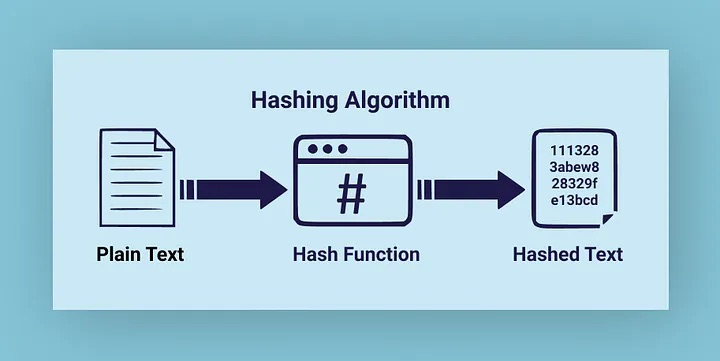
\includegraphics[width=0.5\textwidth]{img/1-img/hash-function.jpeg}
\end{center}
    

\end{frame}


\begin{frame}
\frametitle{Proprietà delle funzioni di hash}

\begin{itemize}
    \item \textbf{Determinismo}: per uno stesso input la funzione restituisce sempre lo stesso output.
    \item \textbf{Velocità}: la funzione deve essere veloce da calcolare.
    \item \textbf{Difficoltà di inversione}: data l'uscita della funzione è computazionalmente difficile trovare l'input.
    \item \textbf{Diffusione}: piccole variazioni nell'input devono produrre grandi variazioni nell'output.
    \item \textbf{Resistenza alle collisioni}: è computazionalmente difficile trovare due input diversi che producano lo stesso output.
\end{itemize}
\end{frame}

\begin{frame}
\frametitle{Preimage resistence}
Prima (debole) resistenza alla preimmagine:
\begin{itemize}
    \item per quasi tutti gli output pre-specificati, è computazionalmente infattibile trovare un qualsiasi input che venga hashato a quell'output.
    Avendo \( y \), è difficile trovare un \( x \) tale che \( h(x) = y \).
\end{itemize}
Seconda (forte) resistenza alla preimmagine:
\begin{itemize}
    \item per un input specificato, è computazionalmente infattibile trovare un altro input che produca lo stesso output.
     Avendo \( x \), è difficile trovare un secondo input \( x' \neq x \) tale che \( h(x) = h(x') \).
\end{itemize}

\end{frame}

\section{Attacchi Sha1}

%------------------------------------------------
\begin{frame}
\frametitle{Primi attacchi a SHA-1}
Nel 2005 il team di ricerca della Shandong University annunciò il primo attacco a SHA-1, con una complessità di \(2^{69}\) operazioni. Pochi mesi dopo fu annunciato un attacco a \(2^{63}\) operazioni.
Un normale attacco che sfrutta il paradosso del compleanno avrebbe una complessità di \(2^{80}\) operazioni.

\vspace{1cm}

Nel 1999 DESCracker era già capace di eseguire \(2^{56}\) operazioni in 56 ore, seguendo la legge di Moore i tempi di calcolo dovevano già essere alla portata di governi e organizzazioni criminali nel 2010.
\end{frame}


\begin{frame}
\frametitle{Google SHAttered}

In 2 anni hanno trovato un modo per generare due PDF diversi con lo stesso hash SHA-1 usando un prefisso specifico per il PDF.
Fino a quel momento l'industria era ancora poco propensa ad abbandonare SHA-1 per la mancanza di un esempio pratico che dimostrasse la collisione.
\begin{itemize}
    \item 9 quantiglioni (\(9,223,372,036,854,775,808\)) di calcoli SHA1 in totale
    \item 6.500 anni di calcolo CPU per completare la prima fase dell'attacco
    \item 110 anni di calcolo GPU per completare la seconda fase 
\end{itemize}

L'attacco SHA-1 shattered è ancora più di 100.000 volte più veloce di un attacco brute force, che rimane impraticabile (\(2^{63}\) operazioni).
\end{frame}

\begin{frame}
\frametitle{Google SHAttered: Come è stato ottenuto}

L'obiettivo è stato quello di trovare coppie di blocchi di dati che, quando \textbf{concatenati con un prefisso P e qualsiasi suffisso S}, producono hash identico.

Si procede trovando la prima coppia di blocchi di dati \(M_{1}^{(1)}, M_{1}^{(2)}\) che portano ad una \textbf{quasi collisione}.

\[
\text{SHA-1} \left( P \parallel M_{1}^{(1)} \parallel M_{2}^{(1)} \parallel S \right) = \text{SHA-1} \left( P \parallel M_{1}^{(2)} \parallel M_{2}^{(2)} \parallel S \right).
\]


Successivamente si sfrutta il primo per trovare un secondo blocco \(M_{2}^{(1)}, M_{2}^{(2)}\) in cui si possa trovare una vera collisione.
La difficoltà di trovare il secondo blocco è significativamente più alta, e spesso richiede più risorse computazionali e strategie sofisticate rispetto al primo.

\end{frame}

\begin{frame}
\frametitle{Creazione del PDF}

Si è poi sfruttata la flessibilità del formato PDF e JPEG per creare i 2 documenti che contenessero i blocchi per generare la collissione.

\begin{center}
    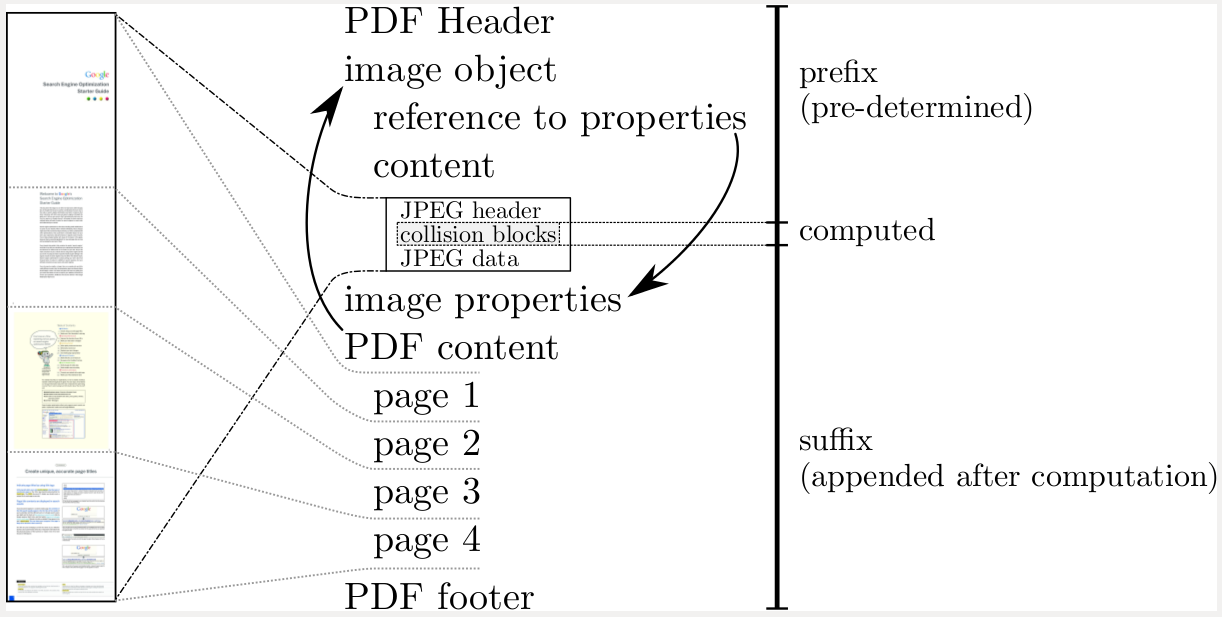
\includegraphics[width=0.8\textwidth]{img/2-img/pdf_format.png}
\end{center}

\end{frame}
\section{Utilizzi funzioni hash}
%------------------------------------------------

\begin{frame}
\frametitle{Secure Hash Algorithm: Iterazioni}

Ogni iterazione usa una funzione non lineare (\textit{f}) e una costante (\textit{k}) che varia a seconda dell'intervallo di iterazione.
La costante k viene successivamente utilizzata all'interno della funzione di compressione.

\begin{itemize}
    \item \textbf{Iterazioni 0-19}: \textit{f = (b and c) or (not b and d)} con \textit{k = 0x5A827999}
    \item \textbf{Iterazioni 20-39}: \textit{f = b xor c xor d} con \textit{k = 0x6ED9EBA1}
    \item \textbf{Iterazioni 40-59}: \textit{f = (b and c) or (b and d) or (c and d)} con \textit{k = 0x8F1BBCDC}
    \item \textbf{Iterazioni 60-79}: \textit{f = b xor c xor d} con \textit{k = 0xCA62C1D6}
    \end{itemize}

\end{frame}

\begin{frame}
\frametitle{Quali utilizzi ci sono per le funzioni hash}
\begin{itemize}
    \item \textbf{Message fingerprint} (integrità dei dati)
    \item \textbf{Password hashing}
    \item \textbf{Digital signature} (solo dell'hash)
    \item \textbf{Entity Authentication/Identification} (meccanismo challenge-response)
    \item \textbf{Message Authentication} (MAC)
    \item \textbf{Encryption} (pseudorandom bit stream)
\end{itemize}
\end{frame}

\begin{frame}
\frametitle{Message Authentication Code (MAC)}

Il MAC (Message Authentication Code) è simile a una firma digitale. 
Quando si riceve un messaggio, si eseguono delle computazioni sul messaggio ricevuto e \textbf{si confronta il risultato con il MAC ricevuto}.

\begin{itemize}
    \item Conoscendo il MAC di un messaggio, è impossibile generare un altro messaggio con lo stesso MAC.
    \item È impossibile trovare due messaggi con lo stesso MAC.
    \item I MAC sono distribuiti uniformemente.
    \item Il MAC deve dipendere da ogni bit del messaggio.
\end{itemize}
\end{frame}

\begin{frame}
\frametitle{H-MAC}

MAC viene generato tramite un meccanismo di crittografia simmetrica, ma esistono anche soluzioni come H-MAC 
che sfruttano una funzione hash.

\vspace{1cm}

H-MAC esegue una funzione di hash due o tre volte a partire da una stessa chiave. In teoria, HMAC potrebbe essere 
calcolato con qualsiasi funzione hash, anche se in pratica si utilizzano quasi sempre SHA-1 o MD5 (entrambi obsoleti).


\end{frame}

\begin{frame}
    \frametitle{H-MAC Parte 2}

H-MAC viene aclcolato a blocchi e a seconda della chiave K bisognerà adattarla alla lunghezza del blocco.

\[
\text{HMAC}(K, M') = H((K' \oplus \text{opad}) \| H((K' \oplus \text{ipad}) \| M'))
\]

Dove $K'$, $\text{opad}$ e $\text{ipad}$ sono costanti.

\end{frame}

\begin{frame}
    \frametitle{Firma digitale con PGP}
PGP calcola un hash dal testo in chiaro, e crea poi da questo hash la firma digitale usando la  \textbf{chiave privata del mittente}.
\begin{center}
    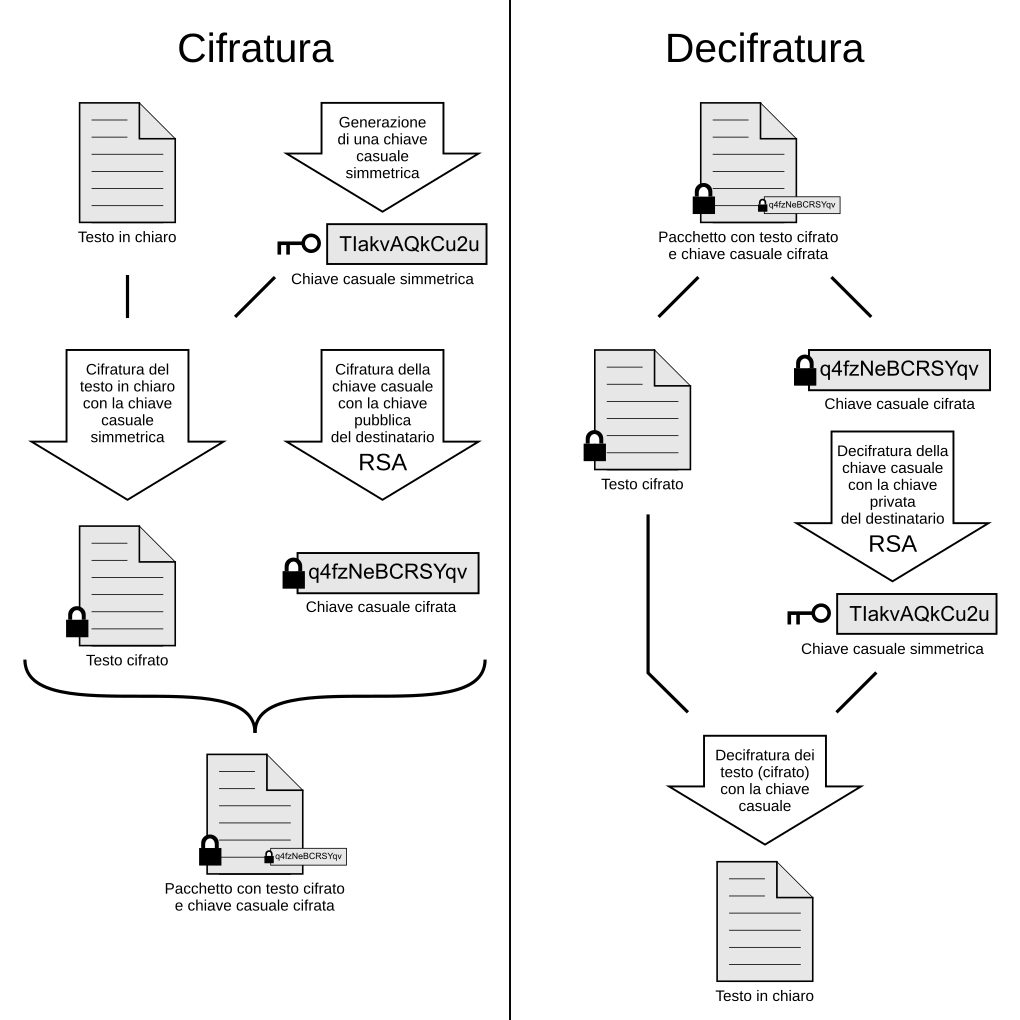
\includegraphics[width=0.5\textwidth]{img/1-img/PGP_diagram_IT.png}
\end{center}
\end{frame}

\begin{frame}
    \frametitle{Firma digitale con PGP Parte 2}
Il destinatario del messaggio calcola il message digest dal testo in chiaro decifrato, e poi usa la \textbf{chiave pubblica del mittente} per decifrare la firma digitale.
Si può verificare la non alterazione del messaggio e l'autenticità del mittente.

\begin{center}
    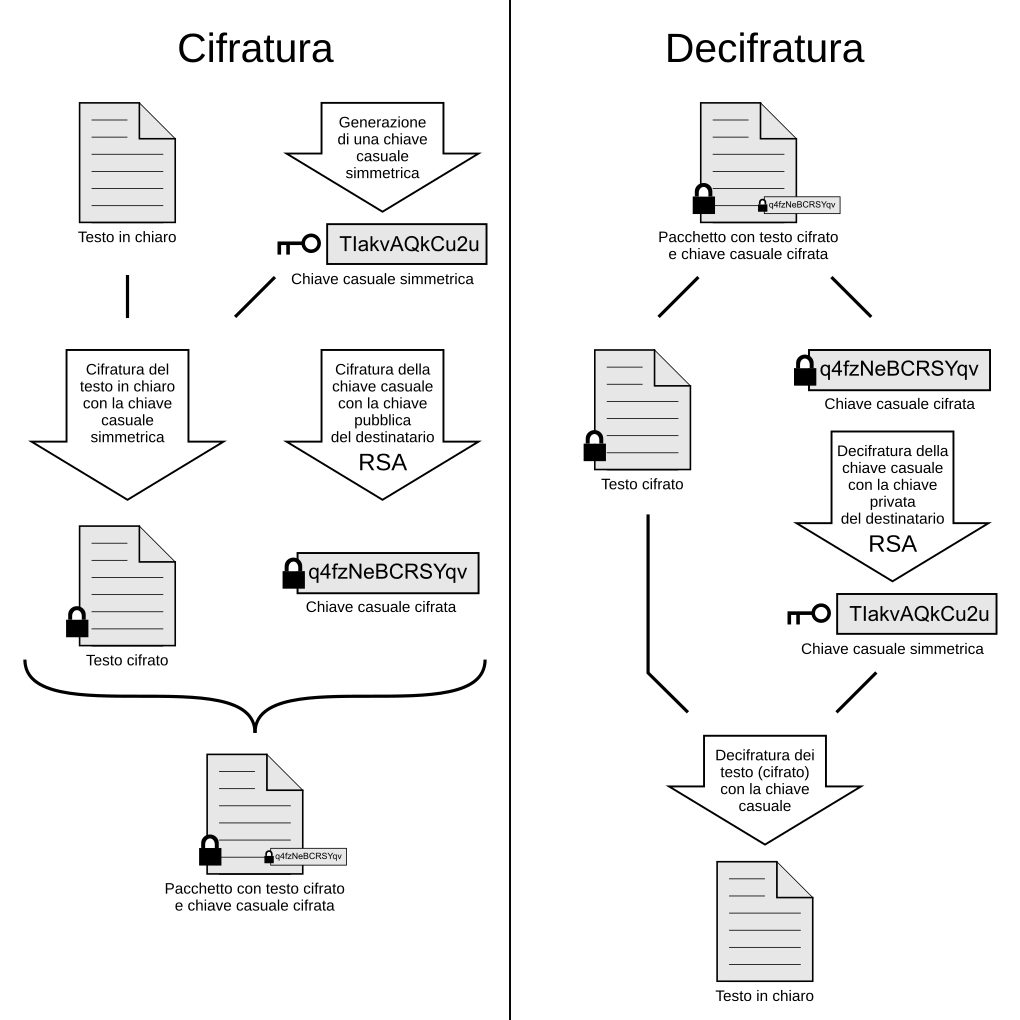
\includegraphics[width=0.5\textwidth]{img/1-img/PGP_diagram_IT.png}
\end{center}
\end{frame}

%----------------------------------------------------------------------------------------
%	CLOSING SLIDE
%----------------------------------------------------------------------------------------

\begin{frame}[plain]
	\begin{center}
		{\Huge Riferimento a fonti esterne:}

	\end{center}
	\begin{itemize}
		\item \href{https://csrc.nist.gov/pubs/fips/180-4/upd1/final}{Link al documento NIST FIPS 180-4}
		\item \href{https://shattered.io}(Google SHA-1 collision: shattered)
		\item \href{https://shattered.io/static/shattered.pdf}{The first collision for full SHA-1}
		\item \href{https://en.wikipedia.org/wiki/SHA-1}{Pseudocodice SHA-1}
		\item \href{https://github.com/clibs/sha1}{Implementazione sha1 in C}
	\end{itemize}
\end{frame}


%----------------------------------------------------------------------------------------

\end{document}